\section{Dataset utilizzato}
Il dataset utilizzato per il progetto è stato prelevato dal sito \cite{dataset_site}, che mette a disposizione i dati di train ($12060$ \textit{sample}) e di test ($647$ \textit{sample}) per lo svolgimento della \textit{challenge}.
Ogni elemento del dataset rappresenta un differente composto chimico ed è caratterizzato da un insieme di $801$ feature dense e oltre $200000$ feature sparse. Considerata la complessità computazionale aggiuntiva derivante dall'utilizzo di queste ultime feature a fronte della minima quantità informazione apportata, è stato deciso di non considerare la porzione sparsa della matrice, come consigliato dal sito citato in precedenza.\\
Ad ogni sample è associato un vettore binario di etichette contenente $12$ elementi. Ognuno di essi corrisponde al risultato di una differente analisi tossicologica a cui la molecola è stata sottoposta. Le analisi effettuate possono essere unite in due macro-gruppi: le prime $7$, identificate dal prefisso \textit{NR}, afferiscono all'area dei test relativi ai \textit{pathways} di segnalazione dei recettori nucleari; le restanti $5$, identificate dal prefisso \textit{SR}, sono relative alla risposta cellulare agli stress.\\
\subsection{Label preprocessing}
L'analisi della matrice delle etichette ha mostrato una discreta presenza di valori \texttt{NaN} (35\% nel train, 10\% nel test); non essendo presente alcuna motivazione di questi valori nella descrizione del dataset, è stato supposto che alcune analisi siano state tralasciate per quelle molecole che i ricercatore hanno ritenuto certamente non tossiche in determinati \textit{pathways}. Per questo motivo, tutti i valori \texttt{NaN} sono stati sostituiti con $0$, rappresentando quindi un esito del test tossicologico negativo per il composto chimico. \\
\todo{capire come inserire grafici distribuzioni etichette}
L'attenzione è stata poi spostata sull'analisi della distribuzione etichette, riportate in Figura , che mostra un forte sbilanciamento tra il numero di 0 ed il numero di 1 per ogni classe. Come già accennato in precedenza, il problema trattato ricade sotto la categoria dei task di classificazione multi-label. Per questo motivo, anche se le classi si sono rivelate sbilanciate, non è stato possibile effettuare operazioni di \textit{over/under-sampling}, in quanto la generazione di un nuovo sample sintetico (o la rimozione di un record nel caso complementare) per una classe avrebbe influenzato lo sbilanciamento delle classi rimanenti. \\
L'analisi della correlazione tra le etichette è stata indagata mediante una rappresentazione \textit{heatmap} della matrice di correlazione, riportata in Figura \ref{fig:labelscorrmatrixheatmap}. I valori di correlazione risultano essere molto bassi in media, salvo per due coppie di label, dove troviamo valori nell'intorno di $0.50$. Analizzando la semantica delle etichette, è emerso che le due coppie di label correlate in modo significativo riguardano l'effetto tossico in un caso sull'intero recettore, nell'altro solo su una porzione di esso.
\begin{figure}
	\centering
	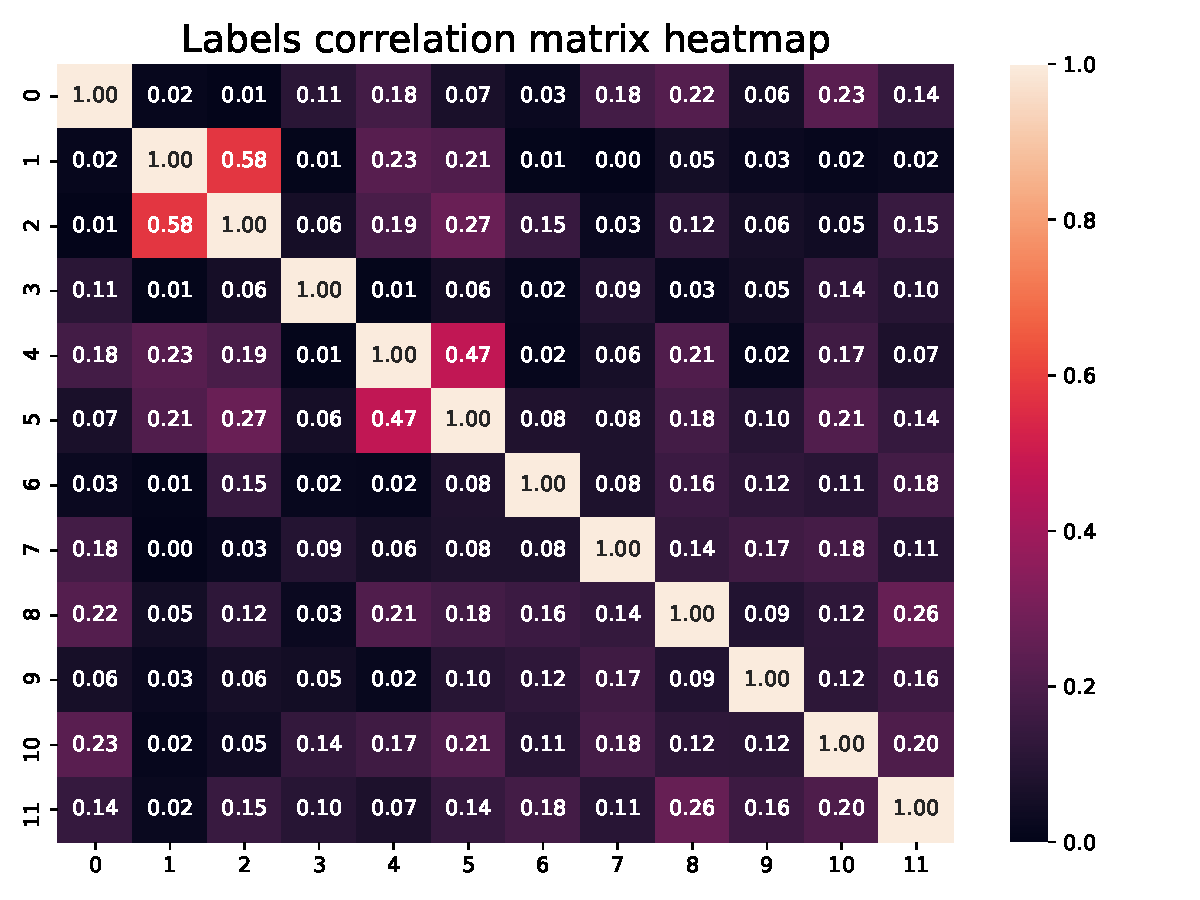
\includegraphics[width=0.7\linewidth]{../images/pdf/labels_corr_matrix_heatmap}
	\caption{Heatmap della matrice di correlazione delle feature. Solo due coppie di feature risultano correlate in modo significativo tra loro.}
	\label{fig:labelscorrmatrixheatmap}
\end{figure}

\subsection{Feature preprocessing}
Per prima cosa è stata verificata la presenza di \textit{missing value} e il tipo dei dati contenuti nella matrice di feature. L'analisi non ha evidenziato la presenza di alcun valore mancante e i dati si sono rivelati tutti di tipo numerico continuo.\\
Sono state eseguite alcune operazioni di pulizia del dataset, rimuovendo $7$ feature (mostravano varianza nulla, quindi erano prive di qualsivoglia informazione) e $425$ oultiler, individuati come quei record che avessero almeno $\frac{1}{4}$ dei valori che eccedessero $3$ volte lo scarto interquantile delle relative feature.\\
L'analisi della correlazione tra feature e label non ha mostrato la presenza di feature altamente correlate alle label, con un valore di correlazione massimo pari a $0.35$; le feature maggiormente correlate alle diverse etichette si sono inoltre rivelate essere tutte differenti (tranne in un caso), rafforzando l'ipotesi di un'assenza di uno stretto legame tra le etichette e un'unica feature.
In Figura \ref{fig:distributionhighcorr} è riportata un'analisi di come le varie feature/etichette risultate altamente correlate($> 0.90$) con altre feature/etichette. È possibile vedere come la larga maggioranza di elementi sia correlato con un basso numero di feature (si noti la scala logaritmica sull'asse x). Troviamo poi un insieme di feature correlate con un numero di elementi compreso tra $5$ e $30$, mentre una decina di feature risultano correlate a più di 40 elementi. Questo suggerisce che sia opportuno eseguire un'operazione di feature reduction prima di eseguire l'addestramento del modello, in modo da ridurre la ridondanza di informazione e velocizzare così sia il processo di train sia quello di inferenza.
\begin{figure}
	\centering
	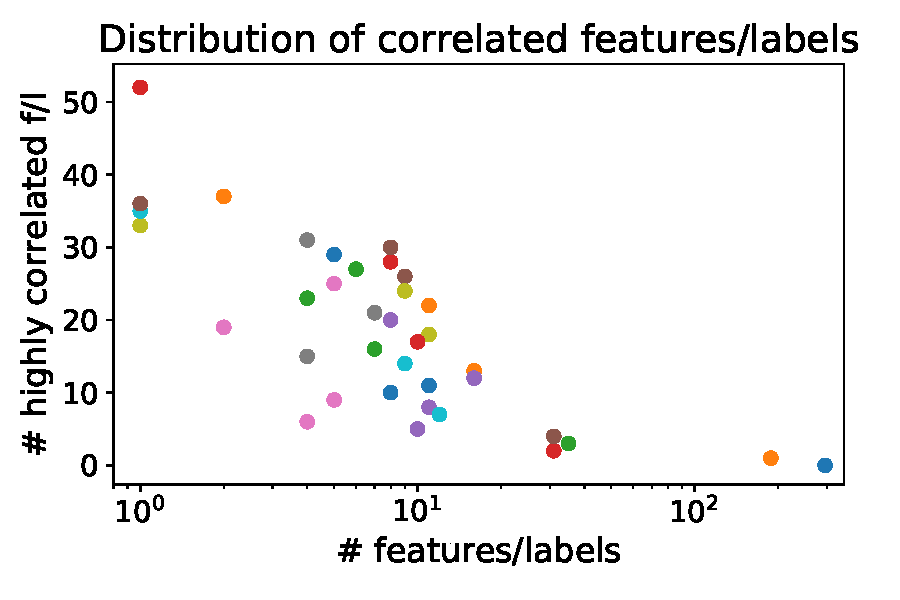
\includegraphics[width=0.7\linewidth]{../images/pdf/distribution_high_corr}
	\caption{Distribuzione di feature/label altamente correlate. È stata utilizzata la scala logaritmica per l'asse x.}
	\label{fig:distributionhighcorr}
\end{figure}
Infine, I dati sono stati  standardizzati con media nulla e deviazione standard unitaria, in modo da non creare squilibri nell'input dei modelli neurali presentati nelle prossime sezioni; ciò è stato fatto in quanto feature con scale differenti possono portare instabilità nella rete, causando la creazione di pesi troppo elevati che rendono la computazione fortemente suscettibile a piccole variazioni dell'input.